% Time-memory-data cryptanalysis of the HiTag2 stream cipher
%
% Presentation file
% Rajesh Bachani

\documentclass{beamer}
\setbeamertemplate{navigation symbols}{}

\usepackage[english]{babel}
\usepackage[latin1]{inputenc}
\usepackage{graphicx}
\usepackage{colortbl}
\usepackage{url}
\usepackage{beamerthemeshadow}
\usepackage[english]{babel}
% or whatever

\usepackage[latin1]{inputenc}
% or whatever

\mode<presentation>
{
  \usetheme{Warsaw}
  % or ...

  \setbeamercovered{transparent}
  % or whatever (possibly just delete it)
}

% Delete this, if you do not want the table of contents to pop up at
% the beginning of each subsection:
\AtBeginSubsection[]
{
  \begin{frame}<beamer>{Outline}
    \tableofcontents[currentsection,currentsubsection]
  \end{frame}
}

% If you wish to uncover everything in a step-wise fashion, uncomment
% the following command: 

%\beamerdefaultoverlayspecification{<+->}


% the document begins here

\begin{document}
\title{Time-memory-data cryptanalysis of the HiTag2 stream cipher}
\subtitle{M.Sc. project presentation}

\author{Rajesh Bachani}

\institute
{
  Department of Mathematics\\
  Technical University of Denmark
}

\date
{
	Supervisor: Dr.~Erik Zenner
}

\begin{frame}
  \titlepage
\end{frame}

\begin{frame}{Outline}
  \tableofcontents
\end{frame}

\section{Introduction}

\subsection{Basics}

\begin{frame}{Cryptography}

  \begin{itemize}
  \item Cryptography provides data confidentiality, integrity, authentication, non-repudiation etc. 
  \item Main ideas: encryption, decryption and `secret key'
  \item Cryptosystems can be symmetric-key or asymmetric-key
  \item Symmetric-key cryptosystems are further divided into two categories: 
  	\begin{itemize}
  		\item Block cipher
  		\item Stream cipher
  	\end{itemize}
  \end{itemize}
\end{frame}

\begin{frame}{One-time pad}
  \begin{itemize}
  \item OTP provides the basic design principle for stream ciphers
  \item A random key is chosen and \textit{xor}'ed with plaintext, bitwise
  \end{itemize}
  
  \begin{figure}[htp]
	\centering
	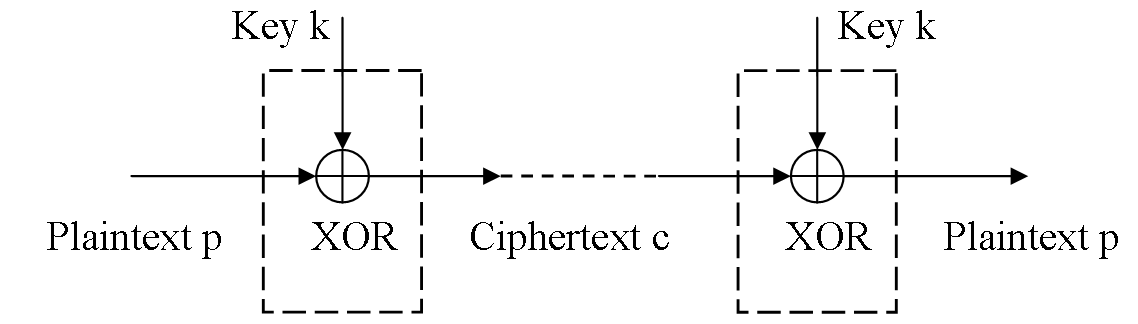
\includegraphics[width = 3in]{./figures/one-time-pad.PNG}
	\end{figure}
	
	\begin{itemize}
		\item OTP exhibit perfect secrecy, but suffer from the following problems:
  	\begin{enumerate}
  		\item Long and random key is required
  		\item Key can be used just once
  	\end{enumerate}
  \end{itemize}
\end{frame}


\begin{frame}{Pseudo-random number generator}
	
	
	\begin{itemize}
		\item PRSG generates a long pseudo-random \textit{keystream} using a short key
		\item The same key can be re-used by using a different initialization parameter for every run of the cipher
	\end{itemize}
	
  \begin{figure}[htp]
	\centering
	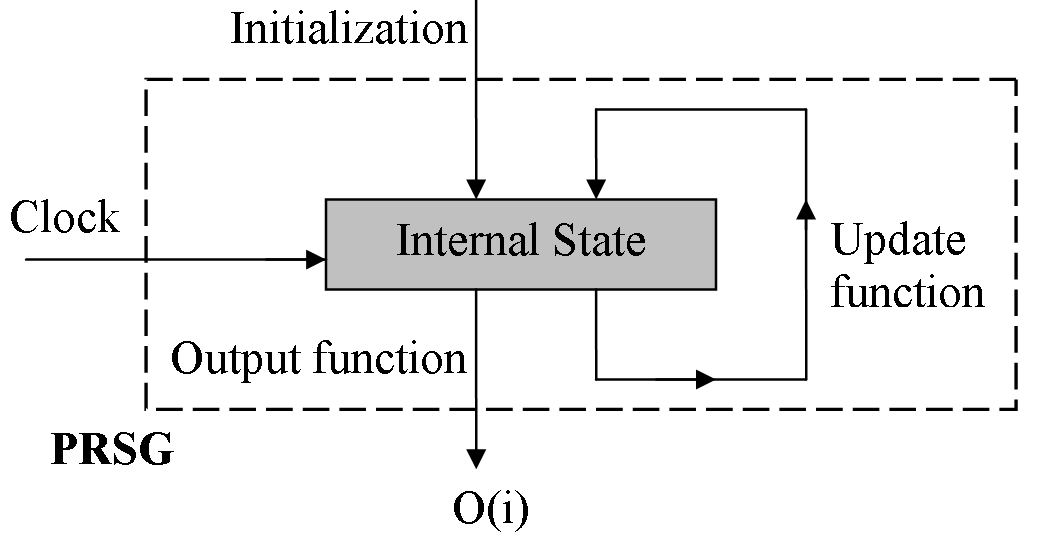
\includegraphics[width = 2.5in]{./figures/prsg.PNG}
	\end{figure}

\end{frame}

\begin{frame}{Internal model of stream cipher}

  \begin{figure}[htp]
	\centering
	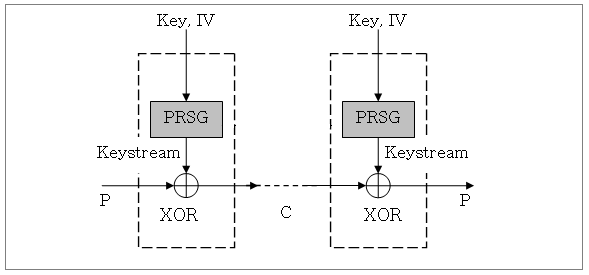
\includegraphics[width = 2.5in]{./figures/stream-cipher.PNG}
	\end{figure}

	\begin{itemize}
		\item The perfect secrecy of OTP does not apply here as the keystream is pseudo-random in nature
	\end{itemize}
\end{frame}

\begin{frame}{Linear feedback shift register}
	\begin{itemize}
		\item Linear feedback shift register (LFSR) is one way to implement PRSG

	\end{itemize}
	\begin{columns}
	
	\begin{column}{5cm}
	\begin{figure}[htp]
	\centering
	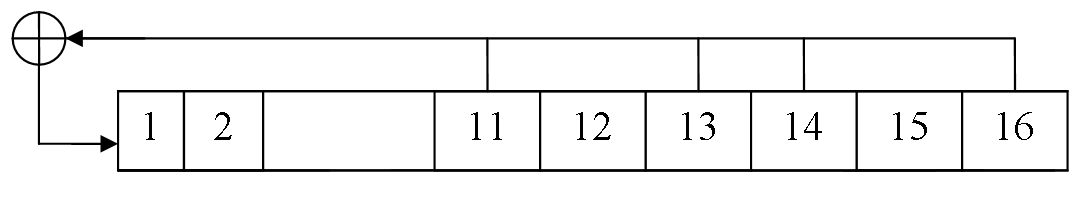
\includegraphics[width = 2in]{./figures/lfsr-example.PNG}
	\end{figure}
	\end{column}
	
	\begin{column}{5cm}
	\begin{figure}[htp]
	\centering
	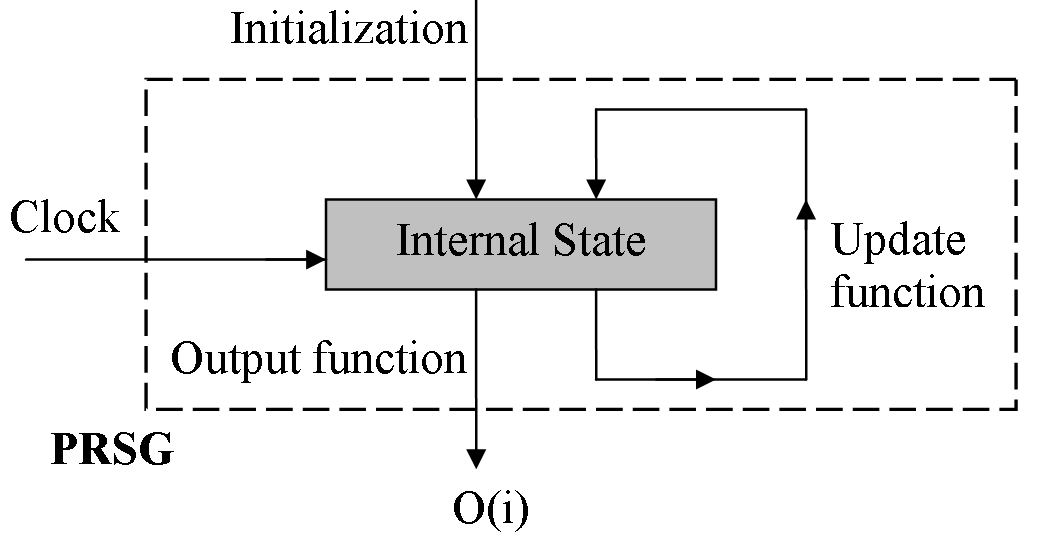
\includegraphics[width = 2in]{./figures/prsg.PNG}
	\end{figure}
	\end{column}	

	\end{columns}
\end{frame}	
	



%\begin{frame}{Make Titles Informative}
%
%  You can create overlays\dots
%  \begin{itemize}
%  \item using the \texttt{pause} command:
%    \begin{itemize}
%    \item
%      First item.
%      \pause
%    \item    
%      Second item.
%    \end{itemize}
%  \item
%    using overlay specifications:
%    \begin{itemize}
%    \item<3->
%      First item.
%    \item<4->
%      Second item.
%    \end{itemize}
%  \item
%    using the general \texttt{uncover} command:
%    \begin{itemize}
%      \uncover<5->{\item
%        First item.}
%      \uncover<6->{\item
%        Second item.}
%    \end{itemize}
%  \end{itemize}
%\end{frame}

\subsection{Time-memory tradeoff attacks}

\begin{frame}{Brute force attack}
\end{frame}

\begin{frame}{Precomputed ciphertext attack}
\end{frame}

\begin{frame}{Tradeoff attack}
\end{frame}

\begin{frame}{Birthday paradox}
\end{frame}

\subsection{HiTag2 stream cipher}

\begin{frame}{Background}
\end{frame}

\begin{frame}{Design}
\end{frame}


\section*{Summary}

\begin{frame}{Summary}

  % Keep the summary *very short*.
  \begin{itemize}
  \item
    The \alert{first main message} of your talk in one or two lines.
  \item
    The \alert{second main message} of your talk in one or two lines.
  \item
    Perhaps a \alert{third message}, but not more than that.
  \end{itemize}
  
  % The following outlook is optional.
  \vskip0pt plus.5fill
  \begin{itemize}
  \item
    Outlook
    \begin{itemize}
    \item
      Something you haven't solved.
    \item
      Something else you haven't solved.
    \end{itemize}
  \end{itemize}
\end{frame}


\end{document}


